%
\section{Magnetospheric Input} \label{cap:magneto_input}
%
The documentation group for the magnetospheric inputs to the TIEGCM model 
consists of Barbara Emery, Wenbin Wang and Yue Deng, with help from others 
as needed.
%
\subsection{Parameters to define the magnetospheric inputs}\label{cap:maginput}
% 
Magnetospheric inputs are the high latitude ion convection model (Heelis or
2005 Weimer) and the aurora, which are described in the following sections.
In version 1.92, the aurora depends on the Hemisphere Power (\code{HP}),
with a minor dependance of the auroral radius on the Cross Polar Cap
Potential (\code{CPCP}).  The Heelis ion convection \cite{heelis1982}
depends on the Cross Polar Cap Potential (\code{CPCP}) and the IMF By.
The input parameters for the 2005 Weimer model \cite{weimer2005}
are solar wind density and speed, and the IMF By and Bz. \\

The potential model is specified in the input file as:
%
\begin{enumerate}
\item POTENTIAL_MODEL = 'NONE'
\item POTENTIAL_MODEL = 'HEELIS'
\item POTENTIAL_MODEL = 'WEIMER05' \\

where 'NONE' means the high-latitude ion drift velocity and electric potential
is zero.  The aurora is specified in the input file as:
%
\begin{enumerate}
\item AURORA = 0
\item AURORA = 1

where 0 means no aurora and '1' means calculate and use a model aurora
(\cite{roble1987}). \\

The magnetospheric input parameters for the convection and auroral models
can be defined in two ways in the namelist input file:
%
\begin{enumerate}
\item Directly specify them in the namelist file as single-valued
parameters under the names of: POWER, CTPOTEN, BYIMF, BZIMF, SWVEL, and SWDEN.
It is possible to specify BXIMF (IMF Bx) also, but this is not used in the
2005 Weimer convection model.  Multiple-valued parameters can be specified
under the names of: POWER_TIME, CTPOTEN_TIME, BYIMF_TIME, BZIMF_TIME,
SWVEL_TIME, and SWDEN_TIME, where four values are given for each
time as: ut_daynumber, ut_hour, ut_minute, value.
\item Specify and use the "\directory{gpi.F}" file (GPI_NCFILE) for the
Heelis ion convection model or the "\directory{imf.F}" (IMF_NCFILE) for
the 2005 Weimer ion convection model in the namelist file, but not both.
It is best to comment out the single- or multiple-valued parameters listed
above when using this option because the default is to use the listed
input namelist values.  The code will stop if CTPOTEN is given and
'WEIMER05' is requested.

The GPI_NCFILE provides 3-h Kp, daily 10.7 cm solar flux data, and 81-day
10.7 cm solar flux data centered on the given day.  The "\directory{gpi.F}"
code calculates \code{HP} and \code{CPCP} from the Kp index. For this case,
in the namelist file, comment out the F107, F107A, POWER, and CTPOTEN
lines, and select POTENTIAL_MODEL = 'HEELIS' and the GPI_NCFILE (a netcdf file).
The formulas are
 \cite{zhang2008}
%
\begin{equation}
  \begin{split}
      \text{if} \quad Kp \leq & 7 \\
                     hp =&  16.82 \cdot e^{(0.32 kp)} - 4.86 \\
      \text{if} \quad Kp >&  7 \\
                     hp =& 153.13 + (kp- \frac{7}{9-7}(300-153.13))
   \end{split}
    \label{eq:maginp_1}
\end{equation}
%
\begin{equation}
  cpcp = 15 + 15 kp + 0.8 kp^2
    \label{eq:maginp_2}
\end{equation}
% 
\end{enumerate}
%
The IMF_NCFILE also provides Kp and 10.7 cm solar flux data, but additionally
provides hourly interplanetary magnetic field (IMF) data and solar wind speed
(Vsw) and density (Dsw).  The satellite IMF and plasma data are time-shifted
to the bow shock nose of the Earth's magnetosphere as described in the
NASA Geophysical Data Center web site for OMNI data at
http://omniweb.gsfc.nasa.gov/ow.html.  All data time-shifted to the bow
shock that lie between 0000 and 0010 UT are used in the hourly average
centerd at 0030 UT.  The "\directory{imf.F}" code interpolates the data
to the model time.  No lag is done between the bow shock and the polar
cap for hourly data, although polar ground magentometer stations respond
between 9 and 25 minutes later (Weimer, 2009 private communication).
When we go to higher resolution IMF and plasma data, then we will add a
lag time between the bow shock and the high-latitude ion convection.
%
If the hourly By, Bz, Vsw, or Dsw are missing in the IMF_NCFILE and
also absent (commented out) in the namelist, then the code will stop
because there is no provision for filling in IMF or plasma gaps.
Since Dsw has little effect on the Weimer 2005 \code{CPCP} as described later,
it can be set in the namelist (SWDEN = 4) to avoid the code stopping during
periods when Dsw is missing.
%
If POWER is absent from the namelist, \code{HP} is calculated from
Emery et al. (2008) \cite{Emery2008} from IMF Bz (in nT) and the solar wind
velocity (Vsw in km/s).  For this case
in the namelist file, comment out the F107, F107A, POWER, CTPOTEN, BXIMF, BYIMF,
BZIMF, SWVEL, and SWDEN
lines, and select POTENTIAL_MODEL = 'WEIMER05' and the IMF_NCFILE (a netcdf file).
The formulas are
 \cite{Emery2008}
%
\begin{equation}
  \begin{split}
      \text{if} \quad Bz <& 0 \\
		     hp = {6.0 + 3.3 \cdot abs(Bz) + (0.06 + 0.003 \cdot abs(Bz)) \cdot
		      (min(Vsw,700) - 300)} \cdot fac \\
      \text{if} \quad Bz \geq&  0 \\
		     hp =& {5.0 + 0.05 \cdot (min(Vsw,700) - 300)} \cdot fac \\
   \end{split}
    \label{eq:maginp_3}
\end{equation}
where fac = 2.0, so the NOAA/DMSP estimated \code{HP} is doubled to
be closer to the GUVI estimated \code{HP}.  Zhang and Paxton (2008)
\cite{zhang2008} show in their Figure 2. that the GUVI energy flux
and the DMSP-F14 energy flux are similar along the cut of the DMSP
satellite, but they show in their Figure 11, that the GUVI estimated
\code{HP} is larger than either the DMSP-F15 estimated \code{HP} or
the NOAA estimated \code{HP}.  Their Figure 8a shows the GUVI \code{HP}
as a function of Kp versus the DMSP \code{HP} from Hardy et al. (1998,
unpublished), which is similar to the intercalibrated NOAA/DMSP \code{HP}
versus Kp in Figure 9 of Emery et al. (2008) \cite{Emery2008}.  Thus,
the factor of 2.0 increase increases the NOAA/DMSP \code{HP} to agree
with the GUVI \code{HP} especially at the higher Kp levels.  In addition,
TIEGCM modeling studies have shown that the auroral energy flux needs
to be increased in order to fit the observed nitric oxide [NO] observations
(private communication S. Solomon and L. Qian).  Finally,
\code{HP} is not allowed to be less than 5.0 GW when calculated from IMF
Bz and Vsw.
%
[NOTE: Weimer 2001 model \cite{Weimer2001} is still in version 1.92.
WHY?  It relies on
calccloc so the calculated convection position is not very good
for Bz positive conditions when abs(By) is less than Bz.
But it could be improved to use the values in 2005.]
%
The order of calls is:
%
\begin{enumerate}
\item Read namelist and open any netcdf input files in module \src{init.F}
\item Advance time-step in module \src{advance.F} and interpolate input
parameters with possible calls to getgpi in module \src{gpi.F} or to
getimf in module \src{imf.F}.  If the potential model is WEIMER (01 or 05),
and POWER is not provided by the namelist, then call hp_from_bz_swvel in
module \src{util.F}.
\item Call aurora_cons in module \src{aurora.F} from module \src{advance.F}
\item Call convection model from module \src{advance.F} (and override auroral
constants found in aurora_cons if the Weimer 2005 model is used)
\item Call module \src{dynamics.F} from module \src{advance.F}, which in turn
calls aurora in module \src{aurora.F}.
% 
\end{enumerate}
%
\subsection{The Heelis convection pattern \index{HEELIS.F}}\label{cap:heelis}
% 
The input to \src{module heelis} is summarized in table
\ref{tab:input_heelis}.
%
\begin{table}[tb]
\begin{tabular}{|p{5cm} ||c|c|c|c|c|c|} \hline
physical field               & variable        & unit&pressure
level& timestep
\\ \hline \hline
%
Radii of convection flow reversal circle &   $\theta_0$ \code{theta0}  & radians  &   & $t_n$\\
Offset between the center of the convection circle and the geomagnetic pole along the geomagnetic noon and
midnight line &  \code{offc}  & radians  &     & $t_n$\\
Offset between the center of the convection circle and the geomagnetic pole along the geomagnetic dawn-dusk 
line &  \code{dskofc}  & radians  &    & $t_n$\\
Potential at the center of the convection circle &  \code{pcen}  &   &	& $t_n$\\
Potential of the evening cell &  \code{psie}  &   &   &\\
Potential of the morning cell &  \code{psie}  &   &   &\\
Daytime entrance of convection in MLT-12 converted to radians & \code{phid}  & radians  &   &\\
Daytime exit of convection in MLT-12 converted to radians & \code{phin}  & radians  &   &\\
Negative departure from phid &  \code{phidm}  &   &   &\\
Positive departure from phid &  \code{phidp}  &   &   &\\
Positive departure from phin &  \code{phinp}  &   &   &\\
Negative departure from phin &  \code{phinm}  &   &   &\\
 &  \code{rr1}  &   &   & \\
Sun's longitude in dipole coordinale (\src{MAGFIELD.F}) &  \code{sunlons}  &   &   & \\
Critical colatitudes (\src{CONS.F}) &  \code{crit}  &   &   &
 \\ \hline
\end{tabular}
\caption{Input fields to \src{module heelis}. All these variables but \code{sunlons}
and \code{crit} are specified in module \index{\src{AURORA.F}}}
\label{tab:input_heelis}
\end{table}
%
The output of module \src{ heelis.F} is summarized in table
\ref{tab:output_heelis}. \\
%
\begin{table}[tb]
\begin{tabular}{|p{3.5cm} ||c|c|c|c|c|c|} \hline
physical field               & variable        & unit&pressure
level& timestep \\ \hline \hline
Fractional presence of dynamo field & \code{Pfrac} (used in \index{\src{dynamo.F}}) &  &  & $t_n$ \\
Heelis potential in geomagnetic coordinates & \code{phihm} (used in \src{dynamo.F}) &  &  & $t_n$ 
\\ \hline \hline
\end{tabular}
\caption{Output fields of module \src{heelis.F}}
\label{tab:output_heelis}
\end{table}
%
\textbf{*Note: the following material is from cite{wang1998}, and 
copyright to the University of Michigan. Some of the material has 
been modified based on the updated TIEGCM}. \\
%
The auroral ion convection pattern in the TIEGCM is 
parameterized using the Heelis model \cite{heelis1982}, 
which is modified to account for IMF By effects on the shape of 
the convection pattern. In general, only two parameters are needed 
to define the auroral ion convection pattern: the cross-tail potential 
$\Phi$ in kilovolts and the interplanetary magnetic field $B_y$ component 
(in nanotesla), where a local variable \code{byloc} is set to the IMF $B_y$
in the range $-11.0 \le byloc \le 7.0$ in the northern hemisphere,
and in the range $-7.0 \le byloc \le 11.$ in the southern hemisphere.
[NOTE: This By range is only correct for NH in aurora_cons, and not for SH!]
In versions earlier than version 1.9, the IMF By dependancy was removed.
Other parameters are set up based on these two
parameters that define the convection pattern. \\
%
The first parameter defined is the radii $\theta_0$ of the convection 
flow reversal circle where the potential peaks  
%
\begin{equation}
  \theta_0 = -3.80^0 + 8.48^0 \Phi^{0.1875}
    \label{eq:maginp_4}
\end{equation}
% 
Where $\Phi$ is the cross polar cap potential (\code{CPCP} in kV). 
The center of the circle is located away from the geomagnetic 
poles by \code{offc} along the magnetic noon-midnight line and \code{dskofc} in the 
dawn-dusk direction  
%
\begin{equation}
  \begin{split}
     \code{offc}   =& 1.1^0 \\
     \code{dskofc} =& -0.08^0- \pm 0.15^0 \code{byloc}
  \end{split}
    \label{eq:maginp_5}
\end{equation}
% 
where $+/-$ applies for southern/northern hemisphere, respectively.
The TIEGCM grid is then
transformed into grid points in the new ion convection 
coordinate system defined by\code{offc}  and \code{dskofc} relative to the 
geomagnetic poles. In this coordinate the auroral 
electric potential is generally expressed as
%
\begin{equation}
  \Psi = G(\theta)F(\phi, \theta)
    \label{eq:maginp_6}
\end{equation}
% 
where $G$ and $F$ represent the strongest latitude and local time 
dependencies, respectively, $\theta$ and $\phi$ correspond to the corrected 
magnetic colatitude and magnetic local time. \\
%
Latitude variations of the potential are represented in the 
TIEGCM by two functions, one describing the variation when 
colatitude is smaller than $\theta_0$, the other one describing the 
variation when colatitude greater than$\theta_0$ . The latitude 
gradient of the potential, and therefore the meridional 
electric field, is discontinuous at $\theta_0$ in the TIEGCM 
implementation of the Heelis model. The TIEGCM neglects a few 
degrees of turnover region around the ion convection reversal 
because of the five-by-five degree grid spacing used in the 
TIEGCM. However, this neglect introduces sharp changes in ion 
velocity and neutral wind near the convection reversal which are 
an obvious discrepancy between the calculated and observed 
convection patterns. In the TIEGCM
%
%\begin{equation}
%  \begin{split}
%    \Psi(\phi,\theta) = & \bigl( \frac{\sin \theta}{\sin \theta_0} \bigr)^{r_1} F(\phi,\theta) 
%             \quad   \text{for}  \theta \gt \theta_0 \\
%    \Psi(\phi,\theta) = & F_3(\phi,\theta)\bigl(\frac{\theta}{\theta_0}\bigr)^3 + 
%        F_2(\phi,\theta)\bigl(\frac{\theta}{\theta_0}\bigr)^2 + 
%	F_1(\phi,\theta))\bigl(\frac{\theta}{\theta_0}\bigr) + \code{pcen}
%	\quad   \text{for}  \theta \le \theta_0
%  \end{split}
%    \label{eq:maginp_6}
%\end{equation}
% 
%
\begin{equation}
  \begin{split}
    \Psi(\phi,\theta) = & \bigl( \frac{\sin \theta}{\sin \theta_0} \bigr)^{r_1} F(\phi,\theta) 
             \quad   \text{for}\quad   \theta > \theta_0 \\
    \Psi(\phi,\theta) = & F_3(\phi,\theta)\bigl(\frac{\theta}{\theta_0}\bigr)^3 + 
        F_2(\phi,\theta)\bigl(\frac{\theta}{\theta_0}\bigr)^2 + 
	F_1(\phi,\theta))\bigl(\frac{\theta}{\theta_0}\bigr) + \code{pcen}
	\quad   \text{for} \quad  \theta \leq \theta_0
  \end{split}
    \label{eq:maginp_7}
\end{equation}
% 
where $r_1 = -2.6, F(\phi,\theta) $,  $F_1(\phi,\theta) $, $F_2(\phi,\theta)$  and  
 $F_3(\phi,\theta)$are functions accounting for the local time 
dependencies of the convection pattern. They are chosen such 
that $\Psi(\phi,\theta)$ is continuous at $\theta_0$,  \
code{pcen}is the potential at the center 
of the convection reversal circle due to the $B_y$ effect
%
\begin{equation}
  \code{pcen} = (-0.168 \pm 0.027 B_y)\Phi
    \label{eq:maginp_8}
\end{equation}
% 
Positive $B_y$ increases the evening cell and
negative $B_y$ enlarges the morning cell in the northern 
hemisphere. The opposite behavior occurs in the 
southern hemisphere. \\
%
The cross tail potential is split between the evening and 
morning potentials \code{psie} and \code{psim}. The evening cell is usually 
larger than the morning cell based on both satellite and 
ground measurements, so the normal split used in the TIEGCM is
%
\begin{equation}
   \code{psim} = 0.44 \Phi \quad
   \code{psie} =-0.56 \Phi
    \label{eq:maginp_9}
\end{equation}
% 
The local magnetic time dependencies are described 
by 6 angles. The longitude $0^o$ (12 MLT) in the TIEGCM 
ion convection coordinate system is defined at noon. 
The longitude is positive when rotating clockwise.  
$\code{phid}$ and $\code{phin}$ are local time angles determining the daytime 
entrance and nighttime exit of the ion convection pattern 
(zero potential line) across the polar cap. Their position 
are also affected by the magnitude and orientation of IMF $B_y$
%
\begin{equation}
   \code{phid} = (9.39 \pm 0.21 \code{byloc} - 12.) 15^o/hr
   \code{phin} = (23.5 \pm 0.15 \code{byloc} - 12.) 15^o/hr
    \label{eq:maginp_10}
\end{equation}
% 
where $\pm$ applies for the southern/northern hemispheres, respectively.
The first expression in each formula is in MLT, where 12 hours is then
subtracted because zero is noon MLT.  The MLT value is converted first to degrees
and then to radians in the code. \\
%
The regions over which the flow paths are not parallel to the 
convection reversal circle are specified by local hour limits 
on either side of the zero potential line. The dayside convergence 
region is called the throat region whereas the region on the nightside 
is the Harang discontinuity. The angular limits of these two convergence 
zones at $\theta_0$ are given by positive and negative departures from \code{phid} and \code{phin}, 
respectively, which are denoted by \code{phidp}, \code{phidm}, \code{phinp} 
and \code{phinm}. Figure \ref{fig:mag_inp_1} is illustration 
of an example of the Heelis model output marked with various parameters. \\
%
It should be noticed that the Heelis model is suitable only 
for IMF $B_z$ negative (southward) conditions. As discussed in 
Chapter \ref{cap:maginput}, when $B_z$ is positive (northward), the ion 
convection patterns can have a configuration quite 
different from the two-cell pattern simulated by the 
Heelis model. Up until now, the latest TIEGCM and TIME-GCM 
still use this simple model for the parameterization of the 
convection pattern.  
%
\begin{figure}
  \centering
  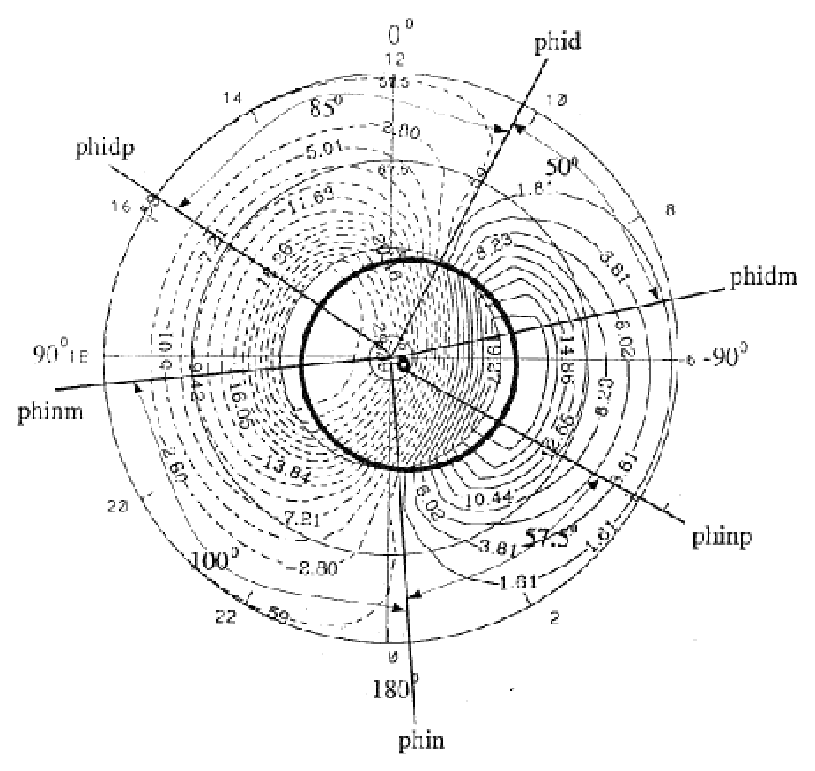
\includegraphics[scale=1.0, angle=0]{./tex_plot/fig2_wenbin.eps}
  \caption{The ion convection pattern (northern hemisphere) for 
  cross-tail potential of 60 KV and the IMF By = 7 nT. 
  Many of the specification parameters are illustrated. }
   \label{fig:mag_inp_1}
\end{figure}
%
%
\subsection{The Weimer convection pattern \index{WEIMER.F}}\label{cap:weimer}
%
The input to module \src{weimer} is summarized in table
\ref{tab:input_weimer}.
%
\begin{table}[tb]
\begin{tabular}{|p{3.5cm} ||c|c|c|c|c|c|} \hline
physical field               & variable        & unit&pressure
level& timestep
\\ \hline \hline
%
UT year, daynumber, hour  &     &   &   & $t_n$\\
Sun's longitude in dipole coordinale (\src{MAGFIELD.F}) &  \code{sunlons}  &   &   & \\
Solar wind density      &     &   &   & $t_n$\\
Solar wind speed        &     &   &   & $t_n$\\
IMF $B_y$, $B_z$ &     & nT  &   & $t_n$\\
 \\ \hline
\end{tabular}
\caption{Input fields to module \src{weimer}.}
\label{tab:input_weimer}
\end{table}
%
The output of module \src{ weimer.F} is summarized in table
\ref{tab:output_weimer}.
%
\begin{table}[tb]
\begin{tabular}{|p{3.5cm} ||c|c|c|c|c|c|} \hline
physical field               & variable        & unit&pressure
level& timestep \\ \hline \hline
Radii of convection flow reversal circle &   $\theta_0$ \code{theta0}  & radians   &   & $t_n$\\
Offset between the center of the convection circle and the geomagnetic pole along the geomagnetic noon and
midnight line &  \code{offc}  & radians  &     & $t_n$\\
Offset between the center of the convection circle and the geomagnetic pole along the geomagnetic dawn-dusk 
line &  \code{dskofc}  & radians   &    & $t_n$\\
Daytime entrance of convection in MLT-12 converted to radians & \code{phid}  & radians  &   &\\
Daytime exit of convection in MLT-12 converted to radians & \code{phin}  & radians  &   &\\
Radii of peak energy flux in the auroral circle &   \code{rrad}  & radians   &   & $t_n$\\
Offset between the center of the auroral circle and the geomagnetic pole along the geomagnetic noon and
midnight line &  \code{offa}  & radians  &     & $t_n$\\
Offset between the center of the auroral circle and the geomagnetic pole along the geomagnetic dawn-dusk
line &  \code{dskofa}  & radians   &    & $t_n$\\
Fractional presence of dynamo field & \code{Pfrac} (used in \index{\src{dynamo.F}}) &  &  & $t_n$ \\
Heelis potential in geomagnetic coordinates & \code{phihm} (used in \src{dynamo.F}) &  &  & $t_n$ 
\\ \hline \hline
\end{tabular}
\caption{Output fields of module \src{weimer.F}.}
\label{tab:output_weimer}
\end{table}
%
The input parameters for the 2005 Weimer model \cite{weimer2005}
are solar wind density (Dsw) and speed (Vsw), and the IMF By and Bz, where the
sign of the IMF By is changed for the potential pattern in the southern
hemisphere.  [ADD A REPRESENTATIVE FIGURE WITH BY LARGE, BZ NEG, NH AND SH?]
The ion convection pattern and the \code{CPCP} are very sensitive to IMF
Bz, IMF By, and Vsw, but \code{CPCP} is relatively insensitive to Dsw.
For example, \code{CPCP} changes from 158 kV to 155 kV for Vsw=450 km,
By=0 nT, and Bz=-15 nT while Dsw increases from 1 cm^-3 and 16 cm^-3
(Maute, 2008 private communication).
Thus, because there are numerous drop-outs of the hourly plasma density Dsw,
we recommend setting the namelist SWDEN = 4 as a constant which is always
used.
%
The output parameters are the Weimer convection circle location variables of
\code{theta0} (set by bndyfitr), \code{offc} (= 4.2^o), and \code{dskofc} (= 0.0^o),
which are set in the 2005 Weimer model, and the convection entrance and exit in
MLT-12 hours converted to radians, \code{phid} and \code{phin} which were calculated
from the Weimer potential patterns.  The auroral circle location variables of
\code{rrad}, \code{offa} (= 4.2^o), and \code{dskofa} (= -2.5^o) are similar to
the parameterizations calculated in \src{aurora.F}, which are discussed in the next
section.
%
%
\subsection{High latitude auroral pattern  \index{AURORA.F}}\label{cap:aurora}
%
% 
The input to module \src{aurora.F} is summarized in table
\ref{tab:input_aurora}.
%
\begin{table}[tb]
\begin{tabular}{|p{3.5cm} ||c|c|c|c|c|c|} \hline
physical field               & variable        & unit&pressure
level& timestep
\\ \hline \hline
%
Cross polar cap potential      &  \code{ctpoten}   &   &   & $t_n$ \\
Hemisphere power      &  \code{power}   &   &   & $t_n$ \\
IMF By      &  \code{byimf}   &   &   &       \\
Sun's longitude in dipole coordinale (\src{magfield.F})      &  \code{sunlons}   &   &   &  
 \\ \hline
\end{tabular}
\caption{Input fields to module \src{aurora}.}
\label{tab:input_aurora}
\end{table}
%
The output of module \src{ aurora.F} is summarized in table
\ref{tab:output_aurora}.
%
\begin{table}[tb]
\begin{tabular}{|p{4cm} ||c|c|c|c|c|c|} \hline
physical field               & variable        & unit &pressure
level& timestep \\ \hline \hline
Radii of the convection flow reversal circle & $\theta_0$ (\code{theta0}) (used in \src{heelis.F}) & radians &  & $t_n$ \\
Offset between the center of the convection circle and 
the geomagnetic pole along the geomagnetic noon and midnight line  & \code{offc} (used in \src{heelis.F}) & radians &  & $t_n$ \\
Offset between the center of the convection circle 
and the geomagnetic pole along the geomagnetic 
dawn-dusk line & \code{dskofc} (used in \src{heelis.F}) & radians  &  & $t_n$ \\
Potential at the center of the convection circle & \code{pcen} (used in \src{heelis.F}) &  &  & $t_n$ \\
Potential of the evening cell & \code{psie} (used in \src{heelis.F}) &  &  & \\
Potential of the morning cell & \code{psie} (used in \src{heelis.F}) &  &  & \\
Daytime entrance of convection in MLT-12 converted to radians & \code{phid}  & radians  &   &\\
Daytime exit of convection in MLT-12 converted to radians & \code{phin}  & radians  &   &\\
Negative departure from phid & \code{phidm} (used in \src{heelis.F}) &  &  & \\
Positive departure from phid & \code{phidp} (used in \src{heelis.F}) &  &  & \\
Positive departure from phin & \code{phinp} (used in \src{heelis.F}) &  &  & \\
Negative departure from phin & \code{phinm} (used in \src{heelis.F}) &  &  & 
\\ \hline \hline
\end{tabular}
\caption{Output fields of module \src{aurora.F}.}
\label{tab:output_aurora}
\end{table}
%
Ion ionization rates and electron heating rate by auroral 
precipitation are added to the total ionization rates 
(variables \code{qo2p, qop, qn2p and qnp}) and electron heating rate 
(variable \code{qteaur}) (solar part is calculated in \index{\src{qrj.F}}) within 
the \src{auroral.F} module itself (subroutine \src{xxxx}), so they are not 
the outputs of the module. \\
%
The precipitation in the \src{auroral.F} module includes electron precipitation, 
soft electron precipitation, cusp precipitation, polar rain (drizzle), and 
ion precipitation. The contribution of each precipitation to ion production 
and electron heating is added to the total ionization and heating rates. \\
%
The auroral parameterizations described in the following sections are
for version 1.9 and later when IMF By effects were restored.
%
\textbf{Note: the following material is from cite{wang1998}, and copyright 
to the University of Michigan. Some of the material has been modified 
based on the updated TIEGCM.}
%
\subsubsection{Electron precipitation  }\label{cap:aurora_elecprecip}
%
The characteristics of the auroral oval used in the TIEGCM are shown 
in Figure \ref{fig:aurora_1}. The oval is circular and is offset
toward the magnetic nighttime by \code{offa}, which is assumed to be $1.0^o$
with the Heelis convection (\code{offc} = $1.1^o$) and $4.2^o$ with the
Weimer 2005 convection (\code{offc} = $4.2^o$).
The aurora is shifted towards the dawn with respect to the convection
reversal circle, and is larger in radius than the convection circle
(e.g. Heelis et al., 1980 \cite{Heelis1980}).
The dawn-dusk offset of the Heelis convection (\code{dskofc}) is related
to the direction and strength of the IMF $B_y$ component and is given by
\ref{eq:maginp_5}.  However, the dawn-dusk offset of the aurora that
goes with the Heelis convection is zero (\code{dskofa} = 0.0^o).  There
is no IMF $B_y$ dependance in the Weimer 2005 convection center location,
so \code{dskofc} = 0.0^o and similarly \code{dskofa} = 0.0^o also for
the location of the aurora.  Thus in both convection cases, the ion
convection center and the center of the auroral oval is away from the
magnetic poles.
%
The TIEGCM defines the auroral oval in a new auroral coordinate 
system with poles in the center of the auroral oval. The width of 
the auroral zone is assumed to be a Gaussian distribution having 
a half-width of the form
%
\begin{equation}
   h = h_0 (1-r_h \cos \lambda )
    \label{eq:aurora_1}
\end{equation}
% 
where $h_0 = 0.5(h_1 + h-2)$, $r_h = \frac{(h_1 - h_2)}{(h_1+h_2)}$ . $\lambda$ is the angle 
clockwise from the entrance of the auroral convection 
throat, which is away from the magnetic local noon by 
an angle of $\chi_h$. $h_1$ (daytime) and $h_2$ (nighttime) are the 
half-widths of the auroral zone at $\lambda = 0^o$ and  $\lambda = 180^o$, respectively, 
and given by
%
\begin{equation}
  \begin{split}
   h_1 =& min(2.35, 0.83 + 0.33 P_1) \notag \\
   h_2 =& 2.5 + 0.025 \cdot max (HP, 55) + 0.01 \cdot min(0,HP-55)
   \end{split}
    \label{eq:aurora_2}
\end{equation}
% 
The angle  $\chi_h$ (variable \code{rroth} in the code, the clockwise 
rotation from noon of dayside $h_1$ Gaussian) is defined as
%
\begin{equation}
   \chi_h = 15^o (0.81 - 0.06 P_1)
    \label{eq:aurora_3}
\end{equation}
% 
where $P_1 = 2.09 ln(H_p)$  is the hemisphere power level, $H_p$ is the 
hemispheric power in unit of GW.  Thus for $P_1 = 1$, the thinnest
auroral width (h1) is at 12 MLT - 0.75 MLT, or at 1115 MLT, while the
maximum auroral width (h2) is 12 hours later at 2315 MLT. \\
%
There is also an angle $\chi_e$ (variable rrote in the code, 
the clockwise rotation from noon of peak dayside energy), 
it is defined as
%
\begin{equation}
   \chi_e = 15^o (0.17 - 0.04 P_1)
    \label{eq:aurora_4}
\end{equation}
%   
Thus for $P_1 = 1$, the least auroral flux (e1) is at 12 MLT - 0.13 MLT,
or at 1152 MLT, while the maximum auroral flux (e2) is 12 hours later
at 2352 MLT. \\
%
\begin{figure}
  \centering
  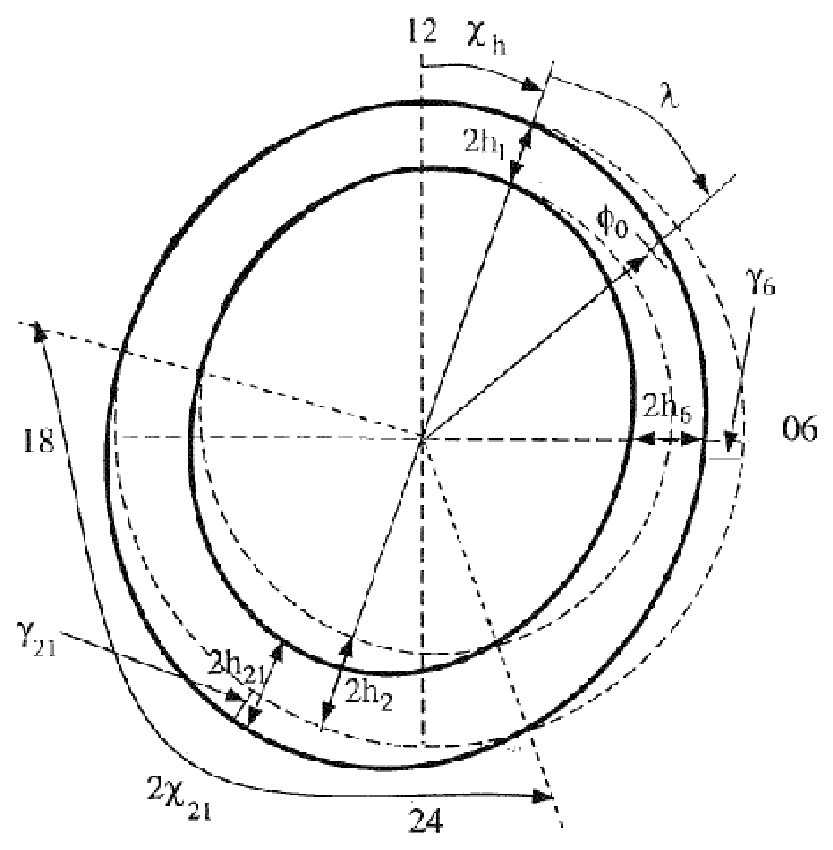
\includegraphics[scale=1.0, angle=0]{./tex_plot/fig3_wenbin.eps}
  \caption{ Illustration of the parameterization of the auroral oval
in the TIGCM - SHOULD REPLACE WITH Roble and Ridley (1987) alfa1,2 fig.)
   \label{fig:aurora_1}
\end{figure}
%
The auroral particle precipitation number flux is then assumed 
to be a product of functions describing the $\lambda$ (longitude) variations 
and a latitudinal Gaussian distribution \cite{roble1987}
%
\begin{equation}
   F = E_0 [1-r_e \cos(\alpha - \chi_e)]exp[-(\frac{\phi-\phi_0}{h})^2]/ 
      (2\alpha_m 1.602 \cdot 10^{-9})
    \label{eq:aurora_5}
\end{equation}
%   
where $\alpha$ is the longitude, $\phi$ is the colatitude in 
the newly defined auroral coordinate system, $\phi_0$ (named \code{arad} 
in the code) is the radii of the auroral oval expressed as
%
\begin{equation}
   \phi_0 = max(-0.43 + 9.69 C_p^0.1875, 14.20 + 0.96 P_l)
    \label{eq:aurora_6}
\end{equation}
%   
where $C_p$ is the cross tail potential in unit of kV and $\alpha_m$
is the characteristic Maxwellian energy of the precipitating particles
in keV and $2\alpha_m$ is the mean Maxwellian energy.
For the Heelis convection, $C_p$ is the same in both hemispheres,
but for the 2005 Weimer convection, $C_p$ is the average of \code{CPCP}
from both hemispheres.
%
The angle $\chi_e$ (variable rrote in the code) is defined in eq:aurora_4
such that
%
\begin{equation}
  \begin{split}
    E_0 [1-r_e \cos(\alpha -\chi_e)] =& E_1 \quad \text{when } \alpha - \chi_e = 0^o \\
    E_0 [1-r_e \cos(\alpha -\chi_e)] =& E_2 \quad  \text{when } \alpha - \chi_e = 180^o
  \end{split}  
    \label{eq:aurora_7}
\end{equation}
%   
where$E_0 = 0.5(E_1+E_2)$  and $r_e = (E_1-E_2)/(E_1+E_2)$. $E_1$ and $E_2$ 
are the energy flux of the precipitating particles (ergs cm-2 s-1) 
in the noon sector and midnight sector, respectively, and given by
%
\begin{equation}
  \begin{split}
    E_1 = & max(0.5, -2.15+0.62 P_1 \notag \\
    E_2 = & 1. + 0.11 H_p 
    \label{eq:aurora_8}
  \end{split}
\end{equation}
%   
The characteristic energy $\alpha_m$ is defined using the 
statistical patterns measured by satellite (e.g. Hardy et al., 1985).
As defined in Roble and Ridley (1987) \cite{roble1987}, there is a
dayside $\alpha_1$ and a nightside $\alpha_2$ that are fixed to the
dayside $E_1$ and nightside $E_2$ energy fluxes rotated by the angle
$\chi_e$.  Since version 1.8, the characteristic Maxwellian electron
energies have been nearly constant at:
%
\begin{equation}
  \begin{split}
    \alpha_1 = 1.5 keV \\
    \alpha_2 = 2.0 keV
    \label{eq:aurora_9}
  \end{split}
\end{equation}
%   
where
\begin{equation}
  \begin{split}
    \alpha_0 = 0.5(\alpha_1+\alpha_2) \\
    r_a = (\alpha_1-\alpha_2)/(\alpha_1+\alpha_2) \\
   F = E_0 [1-r_e \cos(\alpha - \chi_e)]exp[-(\frac{\phi-\phi_0}{h})^2]/ 
    \alpha_m = \alpha_0 \cdot [1 - r_a \cos(\alpha - \chi_e)]
    \label{eq:aurora_8}
  \end{split}
\end{equation}
%%
Thus the characteristic
energy of electron precipitation over the entire auroral oval is not 
changing with geomagnetic storm intensities (i.e. Kp), although Zhang
and Paxton (2008) \cite{zhang2008} show in their Figure 8b that
$2\alpha_m$ increases from 1 keV to 3 keV between Kp 0 and 9 from
GUVI FUV images.
%
\subsubsection{Soft electron precipitation}\label{cap:aurora_softelecprecip}
%
Soft electron precipitation is defined the same as the auroral oval in Section 
\ref{cap:aurora_elecprecip}. At present, it is turned off in the TIEGCM by setting 
the energy flux to be zero (characteristic energy is set to be 75 eV). 
%
\subsubsection{Cusp Electron precipitation}\label{cap:aurora_cuspelecprecip}
%
The polar cusp region is also subject to intense soft particle 
precipitation with an average energy around 100 eV. (The characteristic 
energy (not mean energy!) of the cusp precipitation used in TIEGCM is 
100 eV.) Most of the energy of the precipitating electrons is deposited 
in the F-region, causing localized enhanced electron density and temperature, 
or a so called hot spot (Fontheim et al., 1987; Heikkila and Winningham, 1971). 
The longitude extent of the polar cusp is about 30 to 40 degrees (2-4 MLT hours) 
around magnetic local noon. The polar cusp is more constrained in the latitudinal 
direction with an average width about 2-3 degrees (e.g. Lockwood and Davis, 1995; 
Newell and Meng, 1992), and is located between $75^o$ and $80^o$ magnetic latitudes. 
The location and size of the polar cusp may change dramatically under various 
IMF conditions. \\
%
In the TIEGCM cusp precipitation is parameterized by assuming Gaussian 
distribution in both latitude and longitude. The location of the cusp is 
assumed to be at the daytime convection reversal throat which is determined 
by the strength and direction of the IMF By and Bz components as discussed 
in Section 2.4.2. (???? not there) The Gaussian half width in the longitude direction is $20^o$ 
and the half width in the latitude direction is $5^o$. Thus the TIEGCM, because 
of the limitations of its grid size, overestimates the latitude extent by 
about 5 times as compared to the observed average latitude width of $2^o$ to 
$3^o$ discussed above. One consequence of this parameterization is the 
overestimation of the sizes of enhanced plasma density and temperature 
regions produced by the cusp soft precipitation and, in turn, the 
overestimation of the coupling effect between neutrals and ions, and the 
amount of plasma transported from the dayside ionosphere into the nighttime 
polar cap. \\
%
The typical energy flux of cusp electron precipitation is about 
$0.32 erg/cm^2/s$ varying with geomagnetic and IMF conditions 
(Hardy et al., 1985; Candidi and Meng, 1984; Heikkila and Winningham, 1971). 
In the TIEGCM, the energy flux of the cusp precipitation is given by
%
\begin{equation}
  \begin{split}
      E_c & = 3.12 \times 10^8 (2.4 \times 10^{-1} + 6.7 \times 10^{-3}H_p) \quad  eV/cm^2/s \\
          & = -.5(2.4\times10^{-1} + 6.7\times 10^{-3} H_p) \quad  erg/cm^2/s
  \end{split}
    \label{eq:aurora_12}
\end{equation}
%   
(in TIEGCM 1.9 $E_c$ is defined as 
$(2.4 \times 10^{-1} + 6.7 \times 10^{-3}H_p)/5$ do not know why) 
Thus, the energy flux is $0.14 erg/cm^2/s$ when $H_p = 5.0 GW$ during  magnetic 
quiet times, and $0.63 erg/cm^2/s$ when  is 150.0 GW during a storm.
%
\subsubsection{Polar rain (drizzle)}\label{cap:aurora_polarrain}
%
Spatially homogeneous precipitation of soft particles in the polar cap, 
the so called polar rain, is also included in the TIEGCM. The polar rain 
particles come from the solar corona and get into the upper atmosphere 
through the magnetosheath (Fairfield and Scudder, 1985). The energy fluxes 
of polar rain commonly vary from $10^{-3}$ to $10^{-2} erg/cm^2/s$ (Sotirelis et al., 1997; 
Hardy et al., 1986; Riehl and Hardy, 1986; Gussenhoven et al., 1984; 
Winningham and Heikkila, 1974), although sometimes very strong polar rain 
may occur with energy fluxes up to about $10 erg/cm^2/s$ (Newell and Meng, 
1990, Meng and Kroehl, 1977). The occurrence frequency of polar rain events 
for the IMF Bz southward is about twice that for IMF Bz northward conditions 
(Gussenhoven et al., 1984). Polar rain has strong hemispherical asymmetry, with 
the Earth's north (south) hemisphere favored for away (towards) IMF Bx directions 
(Hardy et al., 1986; Gussenhoven et al., 1984). The energy flux of polar rain also 
has a dawn-dusk gradient controlled by IMF $B_y$ conditions. Polar rain is stronger 
during magnetic storms than during magnetically quiet times 
(Winningham and Heikkila, 1974).  \\
%
The energy spectrum of polar rain can be described by a 
single or by two Maxwellian distributions. The lower energy 
component of polar rain has a very narrow energy distribution 
centered at 80 eV with a standard deviation of 13 eV. The energy 
spectrum of the high energy component has a outstanding peak centered 
at 525 eV but extending over a wide range from 100 eV to several thousand 
eV. The mean energy of the high energy component of the polar rain is about 
1250 eV with a standard deviation of 750 eV (Hardy et al., 1986; 
Riehl and Hardy, 1986). \\
%
In the TIEGCM, polar rain is parameterized by a single 
Maxwellian distribution with a characteristic (not mean energy) 
energy of 500 eV. This simple approach may underestimate the 
contributions of the low energy component of polar rain to the 
ionization rate of the upper atmosphere, while overestimating the 
contributions of the high energy component. The peak altitude of the 
ionization rate is thus moved to lower heights affecting the calculation 
of the F-region electron density in the winter hemisphere polar cap 
greatly. The energy flux and its variations with the geomagnetic
 activity is described in the TIEGCM by
%
\begin{equation}
  \begin{split}
      E_p & = 3.12 \times 10^8 (0.012 + 0.006 H_p) \quad  eV/cm^2/s \\
          & = 0.5(0.012 + 0.006  H_p) \quad  erg/cm^2/s
    \label{eq:aurora_13}
  \end{split}
\end{equation}
%   
%
\subsubsection{Ion precipitation}\label{cap:aurora_ionprecip}
%
Solar proton precipitation inside the polar cap is included in TIEGCM. 
The characteristic energy was assumed to be 10 keV. The energy flux is 
currently set to be 1.E-20, so practically zero. There is also a logical 
variable \code{add\_sproton}, which has a default value of \code{false}. You have
to change this to \code{true} and specify the energy flux \code{e\_sp} if want to 
include this precipitation in the model calculation.
%
\subsubsection{Ion ionization and electron heating rates}\label{cap:aurora_ionelec_heatrates}
%
    It is assumed that particle precipitations has a Maxwellian energy  
    distribution.  The total energy flux is given by 
    (Roble and Rees, 1977; \cite{roble1987})
%
\begin{equation}
      F_E = 2 \alpha F_P
    \label{eq:aurora_14}
\end{equation}
%   
where $F_P$ is the total number flux of the precipitating particles,  
$\alpha$ is characteristic energy of the energy distribution and $2 \alpha$ is the mean 
energy. The ionization rate produced by collisions between 
precipitating particles and neutral particles is then calculated 
using an analytic relationship derived by Lazarev (1967). 
Contributions from both primary and secondary electrons to the 
production of ionospheric plasma are included. The detailed 
description of this calculation is given by \cite{roble1987}. \\
%
The number fluxes of auroral electron precipitation, soft electron 
precipitation and polar drizzle are calculated in the auroral coordinate 
system based on \ref{eq:aurora_14}. The coordinate transfer for each geographic 
grid points, and the final characteristic energies number fluxes 
(variable \code{alfa, alfa2, drizl, flux1, flux2}) and auroral heating 
(\code{qteaur}: used in \src{subroutine \index{settei.F}}) at each grid points are 
calculated in \src{subroutine \index{aurora\_heat}} . \\ 

%
Number flux for the cusp precipitation is obtained in \src{subroutine \index{aurora\_cusp}}.\\

%
The detail of how to obtain ionization rates need to written in detail later. 
( \src{subroutines aurora\_ions, aion and bion}). Formulas need to be added here too.
%


		
